\documentclass[acmtog]{acmart}
\usepackage{graphicx}
\usepackage{subfigure}
\usepackage{natbib}
\usepackage{listings}
\usepackage{bm}

\definecolor{blve}{rgb}{0.3372549 , 0.61176471, 0.83921569}
\definecolor{gr33n}{rgb}{0.29019608, 0.7372549, 0.64705882}
\makeatletter
\lst@InstallKeywords k{class}{classstyle}\slshape{classstyle}{}ld
\makeatother
\lstset{language=C++,
	basicstyle=\ttfamily,
	keywordstyle=\color{blve}\ttfamily,
	stringstyle=\color{red}\ttfamily,
	commentstyle=\color{magenta}\ttfamily,
	morecomment=[l][\color{magenta}]{\#},
	classstyle = \bfseries\color{gr33n}, 
	tabsize=2
}
\lstset{basicstyle=\ttfamily}

% Title portion
\title{Assignment 4:\\ {}} 

\author{Name:\quad Xiaohan Wu  \\ student number:\ 2019533093
\\email:\quad wuxh@shanghaitech.edu.cn}

% Document starts
\begin{document}
\maketitle

\vspace*{2 ex}

\section{Introduction}
\qquad In HW4, we are required to implement Monte-Carlo (single-directional) path tracing for global illumination in the ray-tracing framework. To perform a ray-mesh intersection, we are also required to build a k-d tree as the acceleration structure. The program contains 3 basic parts and 2 optional parts. The three parts are: 1.Implement ray-mesh intersection test with a k-d tree for acceleration. 
2.Implement the ideal diffusion BRDF with an area light source. 
3.Implement the Monte-Carlo path tracing algorithm for global illumination: direct + indirect lighting.The optional parts are:1.Implement the ideal specular and glossy specular BRDF with multiple importance sampling.2.Implement the translucent BRDF with refraction, e.g. glasses and diamonds.
\section{Implementation Details}
\qquad In this section, I will introduce how I implement my program for each part respectively.
\\\indent 1.The realization of K-D Tree is relatively easy after being given the pseudocode shown in Tutorial 7.Here,in addition to changing the judgement of depth being even or not to the judgement of the value of depth mod 3(to evaluate which axis to be devided), I also make a change to choose the median value of the axis instead of the center of the median-triangles along the axis that is devided,which results a relative higher performance.
\begin{figure}[h]
	\centering
	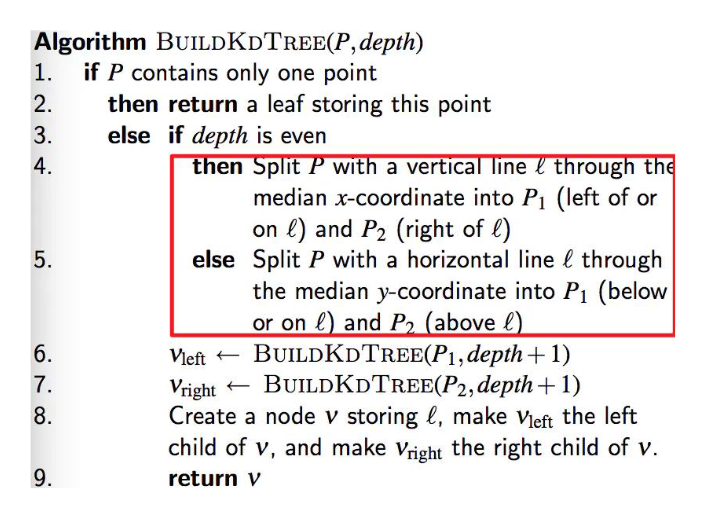
\includegraphics[width=9cm,height=6cm]{KDTREE.PNG}
	\caption{KD-Tree pseudocode}
\end{figure}
\\\indent 2.After implementing KD-tree, here we are going to implement the ideal diffusion BRDF(isotropic diffusion (Lambertian) BRDF), which is different 
from the Phong model used in assignment 3. I use Mally's method here to realize the cosine-weighted hemisphere sampling and calculate the corresponding pdf.
\\\indent 3.After implementing the ideal diffusion BRDF,we need to sample positions on the light surface for area light.Every time, I sample a random position from the unifrom distributionas the default shape of the area light is a rectangle.
\\\indent 4.Then,we can start to render realistic images using Monte-Carlo Path Tracing.For the calculation of each pixel value, I sample 1024 rays with depth 4, and use the iterative implementation of path tracing shown as below.
\begin{figure}[h]
	\centering
	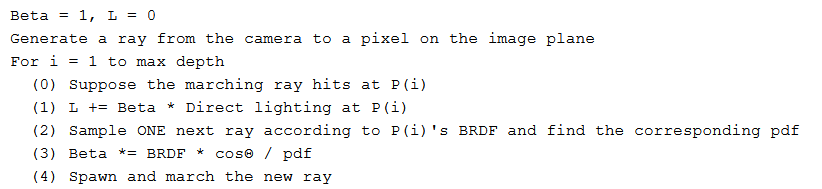
\includegraphics[width=10cm,height=4cm]{Monte-Carlo Path Tracing.PNG}
	\caption{Monte-Carlo Path Tracing}
\end{figure}
\\\indent 5.For the ideal specular part,it's releatively easy to calculate the out direction of the light given the surface normal and the in direction.For the glossy one, according to PBRT, as the definition of glossy is neither specular nor diffusion, so I implement it in the following way:1.Calculating the the ray direction of the ideal specular surface 2. Using cos-weighted sampling to sample around that direction.
\\\indent 6.To realize the ideal tranmission, we need only to calculate the out direction of the ray using Snell's law. One thing that is worth being metioned is that as the ray will not only refract but also reflect in the reality, so I also add the ideal specular into ideal tranmission part to make it seem more real.As we can see in the result part, adding the relectivity will make the short box more translucent compared to the original one.(e.g.the bottom of two boxes.)
\section{Results}
\qquad Below are the results of my programming work.
\begin{figure}[h]
	\centering
	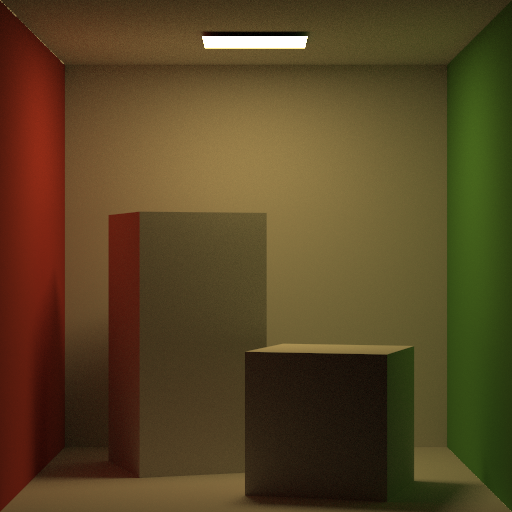
\includegraphics[width=7cm,height=7cm]{output0.png}
\end{figure}
\begin{figure}[h]
	\centering
	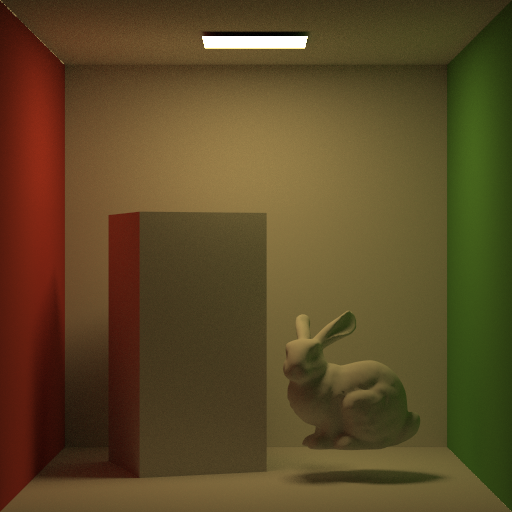
\includegraphics[width=7cm,height=7cm]{output1.png}
\end{figure}
\begin{figure}[h]
	\centering
	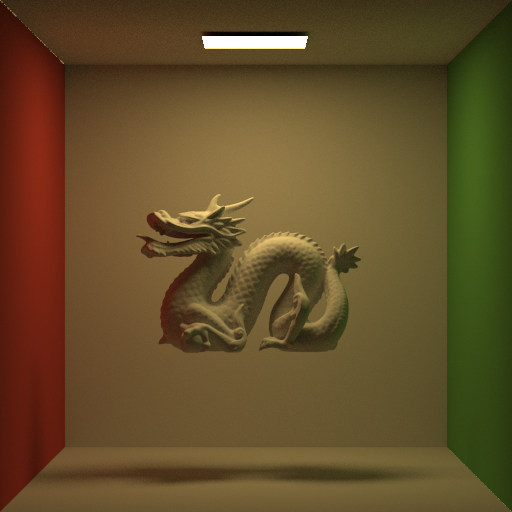
\includegraphics[width=7cm,height=7cm]{output2.png}
\end{figure}
\begin{figure}[h]
	\centering
	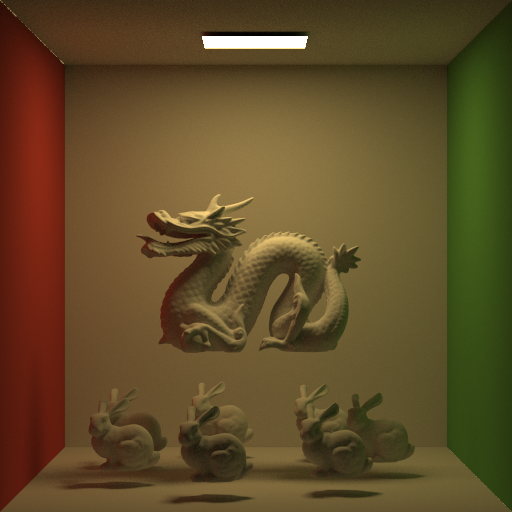
\includegraphics[width=7cm,height=7cm]{output3.png}
\end{figure}
\begin{figure}[h]
	\centering
	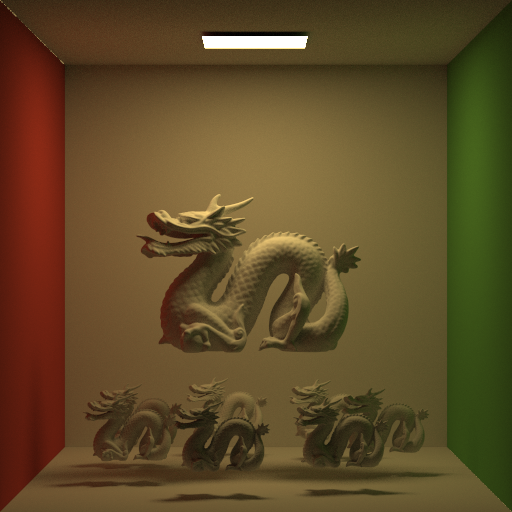
\includegraphics[width=7cm,height=7cm]{output4.png}
\end{figure}
\begin{figure}[h]
	\centering
	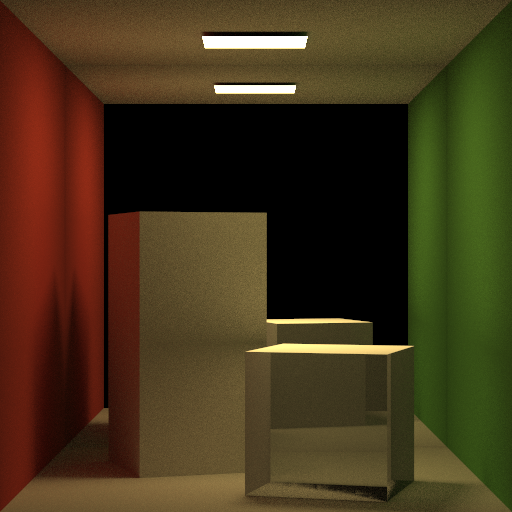
\includegraphics[width=7cm,height=7cm]{spec.PNG}
	\caption{SpecularWall}
\end{figure}
\begin{figure}[h]
	\centering
	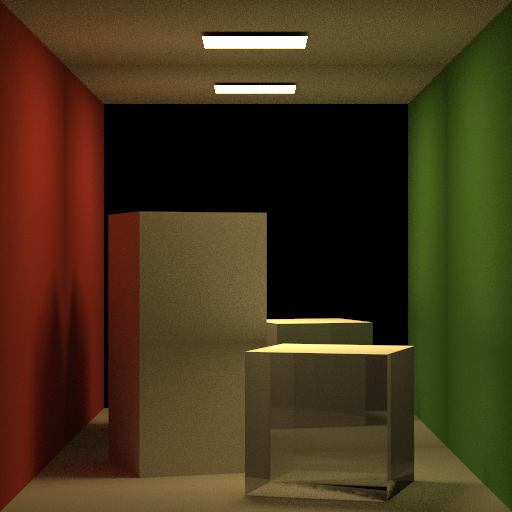
\includegraphics[width=7cm,height=7cm]{spec_reflect.PNG}
	\caption{SpecularWall with reflectivity}
\end{figure}
\begin{figure}[h]
	\centering
	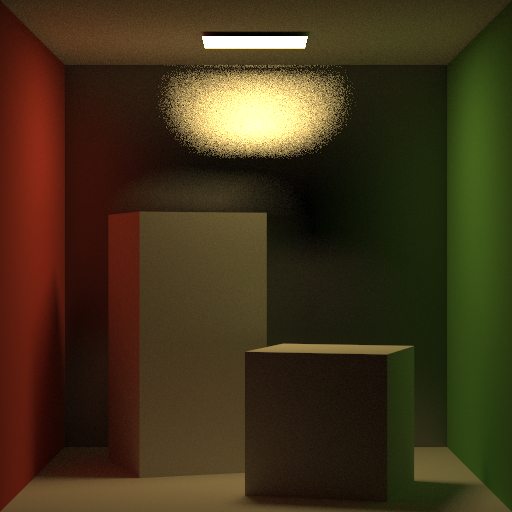
\includegraphics[width=7cm,height=7cm]{glossy.png}
	\caption{glossywall}
\end{figure}
\begin{figure}[h]
	\centering
	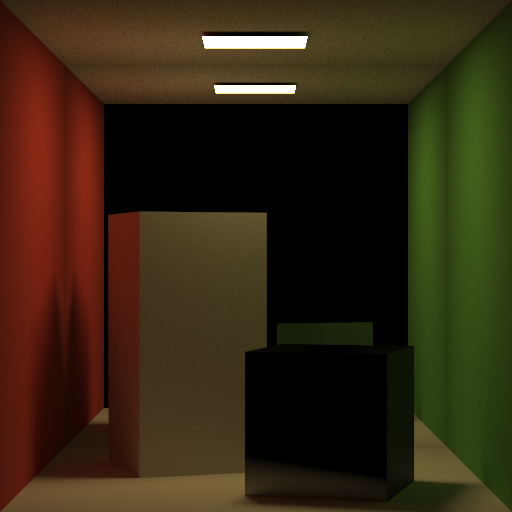
\includegraphics[width=7cm,height=7cm]{box_glossy.png}
	\caption{glossybox}
\end{figure}
\begin{figure}[h]
	\centering
	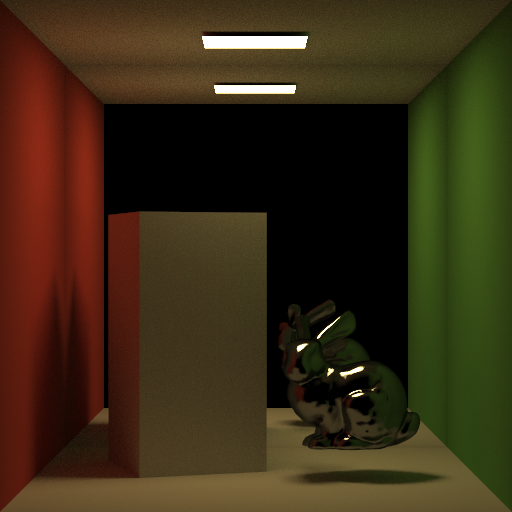
\includegraphics[width=7cm,height=7cm]{bunny_glossy.png}
	\caption{glossybunny}
\end{figure}


\end{document}
